% -	-	-	-	-	-	-	-	-	- %
%% -	-	-	- Trees for Baez' operads -	-	-      - %%

\begin{defn}\label{def-tree}
	An $n-$\emph{tree} is the data $(V, E, s, t)$ where
	\begin{itemize}
		\item $V$ is a finite set of \emph{vertices},
		\item $E$ is a finite set of \emph{edges},
		\item $s : E \to V \cup [1..n]$ is the
			\emph{source map}\footnote{Here we're using the
			comprehension $[a..b] :=
			\{t \in \ZZ \ | \ a \leq t \leq b\}$}, and
		\item $t : E \to V \cup \{0\}$ is the \emph{target map}.
	\end{itemize}
	This data is restricted to satisfy the following conditions:
	\begin{enumerate}
		\item It defines a graph-theoretic tree with vertices
			$V \cup [0..n]$ and edges $E$.
		\item There is exactly one $e \in E$ such that $t(e) = 0$.
	\end{enumerate}
	We use $u \to^{e} v$ to denote\footnote{Since the vertices and
	edges form a tree,  specifying the edge is redundant. We will keep
	this definition for the time being in order to fluidly converse
	with the authors.} that $e \in E$ has source $u$ and target $v$.
\end{defn}

\begin{defn}\label{tree-iso}
	We say that the trees $(V,E,s,t)$ and $(V',E',s',t)$ are
	\emph{isomorphic} if there exist bijections $F_0 : V \cup [0..n]
	\to V' \cup [0..n]$ and $F_1 : E \to E'$ such that
	\begin{eqnarray}
		F_0 s &=& s' F_1 \ \ \ \text{and} \\
		F_0 t &=& t' F_1.
	\end{eqnarray}
	In other words, two $n-$trees are isomorphic if they are equal
	modulo renaming of their vertices and edges.
\end{defn}

\begin{defn}\label{tree-v}
	This is some vocabulary associated with $n-$trees:
	\begin{itemize}
		\item The \emph{children} of the vertex $v$ are the
			elements of $t^{-1} \ \{ v \}$, and the cardinality
			of this set is the \emph{arity} of $v$.
		\item A 0-ary vertex is called a \emph{terminus}.
		\item A tree with one vertex is called a \emph{corolla}.
		\item The edge whose target is the root, and the edges
			whose sources are the leaves, are called
			\emph{external edges}, and the remaining edges are
			the \emph{internal edges}.
	\end{itemize}
\end{defn}

We now define planar trees.

\begin{defn}[Planar trees]\label{plts}
	A \emph{planar $n-$tree} is an $n-$tree such that each vertex is equipped with a linear ordering on the set of its children. An \emph{isomorphism} of such trees is one that preserves the linear orderings.
\end{defn}

We now define trees with lengths.

\begin{defn}[Trees with lengths]\label{twl}
	An $n-$tree \emph{with lengths} is the data $(T,l)$ where $T$ is an $n-$tree and $l : E \to [0, \infty[$. The \emph{length function} $l$ clearly makes $T$ into a planar tree.
\end{defn}

\begin{defn}[Phylogenetic trees]\label{phts}
	A \emph{phylogenetic $n-$tree} is an isomorphism class of $n-$trees with lengths satisfying the following conditions:
	\begin{enumerate}
		\item \emph{There are no unary vertices nor termini}, and
		\item \emph{There are no internal edges of length 0}.
	\end{enumerate}
\end{defn}

A drawing:

\begin{center}
	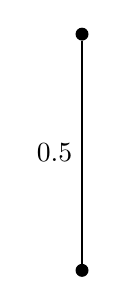
\begin{tikzpicture}[auto]
		\node[circle, draw, fill, inner sep=0pt, minimum size=1.5mm] (1) at (0,0) {};
		\node[circle, draw, fill, inner sep=0pt, minimum size=1.5mm] (2) at (0,3) {};

		\draw (1) to node {0.5} (2);
	\end{tikzpicture}
\end{center}

% green!50!black produces a dark green.

Was it successful?

Now Java code:

\lstinputlisting[language=Java, firstline=1, lastline=4]{inJava.java}

Successful?

% % - Definitions are maybe too conversational.
